\documentclass[twoside]{article}

%
% ADD PACKAGES here:
%

\usepackage{amsmath,amsfonts,graphicx}
\usepackage[letterpaper, margin=1in]{geometry}
\usepackage{url}
\usepackage[hidelinks]{hyperref}
% Imports for writing pseudocode
\usepackage{algorithm}
\usepackage{listings}
\usepackage{xcolor}
\usepackage{graphicx,xspace}
\usepackage{enumerate}
\usepackage{enumitem}
\usepackage{booktabs}
\usepackage[labelfont=bf, font=bf]{caption}
\usepackage{mathtools}
\usepackage{tikz}
\usepackage{float}
\usepackage[colorinlistoftodos]{todonotes}
\definecolor{codegreen}{rgb}{0,0.6,0}
\definecolor{codegray}{rgb}{0.2,0.2,0.2}
\definecolor{background}{rgb}{0.95,0.95,0.92}
\lstdefinestyle{mystyle}{
    backgroundcolor=\color{background},
    commentstyle=\color{codegreen},
    keywordstyle=\color{blue},
    numberstyle=\tiny\color{codegray},
    basicstyle=\footnotesize,
    breakatwhitespace=false,
    breaklines=true,
    captionpos=b,
    keepspaces=true,
    numbers=left,
    numbersep=5pt,
    showspaces=false,
    showstringspaces=false,
    showtabs=false,
    tabsize=2
}
\lstset{style=mystyle}

%
% The following commands set up the lecnum (lecture number)
% counter and make various numbering schemes work relative
% to the lecture number.
%
\newcounter{lecnum}
\renewcommand{\thepage}{\thelecnum-\arabic{page}}
\renewcommand{\thesection}{\thelecnum.\arabic{section}}
\renewcommand{\theequation}{\thelecnum.\arabic{equation}}
\renewcommand{\thefigure}{\thelecnum.\arabic{figure}}
\renewcommand{\thetable}{\thelecnum.\arabic{table}}

%
% The following macro is used to generate the header.
%
\newcommand{\lecture}[4]{
   \pagestyle{myheadings}
   \thispagestyle{plain}
   \newpage
   \setcounter{lecnum}{#1}
   \setcounter{page}{1}
   \noindent
   \begin{center}
   \framebox{
      \vbox{\vspace{2mm}
    \hbox to 6.28in {{\bf CS 244	\hfill Spring 16-17}}
       \vspace{4mm}
       \hbox to 6.28in { {\Large \hfill Assignment #1: #2  \hfill} }
       \vspace{2mm}
       \hbox to 6.28in { {\it Professors: #3 \hfill Students: #4\/} }
      \vspace{2mm}}
   }
   \end{center}
   \markboth{Assignment #1: #2}{Assignment #1: #2}
}

%Use this command for a figure; it puts a figure in wherever you want it.
%usage: \fig{NUMBER}{SPACE-IN-INCHES}{CAPTION}
\newcommand{\fig}[3]{
			\vspace{#2}
			\begin{center}
			Figure \thelecnum.#1:~#3
			\end{center}
	}
% Use these for theorems, lemmas, proofs, etc.
\newtheorem{theorem}{Theorem}[lecnum]
\newtheorem{lemma}[theorem]{Lemma}
\newtheorem{proposition}[theorem]{Proposition}
\newtheorem{question}[theorem]{Question}
\newtheorem{claim}[theorem]{Claim}
\newtheorem{corollary}[theorem]{Corollary}
\newtheorem{definition}[theorem]{Definition}
\newenvironment{proof}{{\bf Proof:}}{\hfill\rule{2mm}{2mm}}

% **** IF YOU WANT TO DEFINE ADDITIONAL MACROS FOR YOURSELF, PUT THEM HERE:
%Numbered environment
\newcounter{example}[section]
\newenvironment{example}[1][]{\refstepcounter{example}\par\medskip
   \noindent \textbf{Example~\thelecnum.\theexample. #1} \rmfamily}{\medskip}

\newcommand{\specialcell}[2][c]{%
 \begin{tabular}[#1]{@{}c@{}}#2\end{tabular}}

\newcommand\E{\mathbb{E}}

\begin{document}
%FILL IN THE RIGHT INFO.
%\lecture{**LECTURE-NUMBER**}{**TOPIC**}{**LECTURER**}{**SCRIBE**}
\lecture{2}{Congestion Control Contest}{K. Winstein \& S. Katti}{Jervis Muindi \& Luke Hsiao}

% **** YOUR NOTES GO HERE:

% Some general latex examples and examples making use of the
% macros follow.
%**** IN GENERAL, BE BRIEF. LONG SCRIBE NOTES, NO MATTER HOW WELL WRITTEN,
%**** ARE NEVER READ BY ANYBODY.

% \begin{figure}[H]
%   \caption{Example Cellphone SoC\label{fig:cell_soc}}
%   \centering
%     \includegraphics[page=5, trim={3cm 4cm 3cm 5.12cm}, clip, width=0.7\textwidth ]{lectures/07-flash-slides.pdf}
% \end{figure}

% \begin{algorithm}
% \caption{Discover Victim Cache}\label{victim}
% \begin{lstlisting}[language=C]
% char A[1024 * 64] = initialized;
%
% int baseline () {
%   sum = 0
%   // fill up cache with the first 32KB of A's data
%   for (int i = 0; i < 1024*32; i++) {
%   	sum += A[i];
%   }
%   sum += A[1024 * 32]; // cause cache conflict, load from main memory
%   return sum;
% }
% \end{lstlisting}
% \end{algorithm}


\section*{Exercise A}

\begin{question}
  Vary the fixed window size by editing controller.cc to see what happens.
  Make a 2D graph of throughput vs. 95-percentile signal delay (similar to what
  is seen on the contest analysis URLs) as you vary this value. What is the
  best single window size that you can find to maximize the overall ``score''
  (log throughput/delay)? How repeatable are the measurements taken with the
  same window size over multiple runs?
\end{question}

We tried several different windows sizes in increments of 5 datagrams. The raw
numbers are shown in Table~\ref{tab:fixed_window}. Score is calculated as
$throughput / delay$, and the best score is shown in bold.

\begin{table}[h]
  \centering
  \caption{Throughput and Delay vs Fixed Window Size}
  \label{tab:fixed_window}
  \scriptsize
\begin{tabular}{rrrr}
  \toprule
  \textbf{\specialcell{Window\\Size}} & \textbf{\specialcell{Throughput\\(Mbits/s)}} & \textbf{\specialcell{95\% Signal\\Delay (ms)}} & \textbf{Score}\\
  \midrule
  5                           & 1.05          & 109          & 9.63           \\
  10                          & 1.93          & 155          & 12.45          \\
  \textbf{15}                 & \textbf{2.66} & \textbf{212} & \textbf{12.55} \\
  20                          & 3.26          & 277          & 11.77          \\
  25                          & 3.73          & 343          & 10.87          \\
  30                          & 4.07          & 401          & 10.15          \\
  35                          & 4.32          & 453          & 9.54           \\
  40                          & 4.51          & 504          & 8.95           \\
  45                          & 4.65          & 557          & 8.35           \\
  50                          & 4.76          & 607          & 7.84           \\
  55                          & 4.85          & 652          & 7.44           \\
  60                          & 4.91          & 711          & 6.91           \\
  65                          & 4.94          & 763          & 6.48           \\
  70                          & 4.96          & 808          & 6.13           \\
  75                          & 4.98          & 855          & 5.82           \\
  80                          & 4.99          & 896          & 5.57           \\
  85                          & 5.00          & 935          & 5.34           \\
  90                          & 5.00          & 972          & 5.14           \\
  \bottomrule
\end{tabular}
\end{table}

These values are plotted as a 2D graph of throughput vs 95-percentile signal
delay in Figure~\ref{fig:exa}.

\begin{figure}[h]
  \centering
  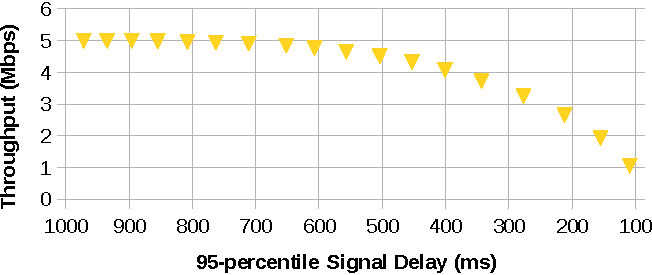
\includegraphics[height=3cm]{./img/exa_fig.pdf}
  \caption{Throughput vs 95-percentile Signal Delay for varying fixed window size.}
  \label{fig:exa}
\end{figure}

To answer the questions, we found that the best score was at a fixed window
size of about 15 datagrams. The measurements taken with the same window size
over multiple runs were very repeatable in the mahimahi environment. The
throughput and delay only varied slightly (i.e. $\pm$ a few hundredths of Mbps
or a few ms).

\vfill
\pagebreak

\section*{Exercise B}
\begin{question}
  Implement a simple AIMD scheme, similar to TCP's congestion-avoidance phase.
  How well does this work? What constants did you choose?
\end{question}

For this exercise, we implemented a simple AIMD protocol, which increments the
\texttt{cwnd} by $alpha/cwnd$ on each ack, and decreases the window by
\texttt{beta} on a loss event (i.e. $cwnd = cwnd / beta$).
This mimics the AIMD behavior of TCP in congestion avoidance.
In our mahimahi environment, there is no loss, and there is unbounded queues.
Thus, to signal when a multiplicative decrease should occur, we use a fixed
timeout value as a signal. We set the timeout to 80ms, which is approximately
the 95-percentile signal delay on the top algorithms from the leaderboard.
We also set the initial congestion window size to 10.

We tried a few of different values for \texttt{alpha} and \texttt{beta},
and recorded their performance in Table~\ref{tab:aimd}.
We found that the typical values of $\texttt{alpha} = 1$ and $\texttt{beta} = 2$
perform worse than many of the fixed window sizes we tested in Exercise A.
In particular, AIMD increased latency as the algorithm tries to slowly use
all the throughput available. We then tweaked the constants to see how being
more aggressive or timid is growth and decrease affected the power score.

\begin{table}[h]
  \centering
  \caption{Throughput and Delay for various AIMD constants}
  \label{tab:aimd}
  \scriptsize
  \begin{tabular}{rrrrr}
    \toprule
    \textbf{Alpha} & \textbf{Beta} & \textbf{\specialcell{Throughput\\(Mbits/s)}} & \textbf{\specialcell{95\% Signal\\Delay (ms)}} & \textbf{Score}\\
    \midrule
    1              & 2             & 4.72          & 847          & 5.57           \\
    1              & 3             & 4.68          & 765          & 6.12           \\
    1              & 4             & 4.65          & 734          & 6.34           \\
    1              & 5             & 4.64          & 724          & 6.41           \\
    1              & 10            & 4.59          & 705          & 6.51           \\
    0.1            & 1.1           & 3.80          & 377          & 10.08          \\
    \textbf{0.1}  & \textbf{1.5}  & \textbf{2.72} & \textbf{142} & \textbf{19.16} \\
    0.1            & 2             & 2.43          & 186          & 13.06          \\
    0.5            & 2             & 4.41          & 570          & 7.74           \\
    0.2            & 4             & 3.23          & 267          & 12.10          \\
    2              & 2             & 4.88          & 1190         & 4.10           \\
    4              & 2             & 4.96          & 1655         & 3.00           \\
    4              & 10            & 4.95          & 1533         & 3.23           \\
    \bottomrule
  \end{tabular}
\end{table}

In general, we found that a slow additive increase (with $\texttt{alpha} < 1$),
combined with a passive multiplicative decrease ($\texttt{beta} < 2$) provided
a better power score on this cellular link that other configurations we tested.
However, even in this best case, only about half of the available throughput was
utilized. Even with the best constant values we found (shown in bold in the
table) are not optimal.

\begin{figure}[h]
  \centering
  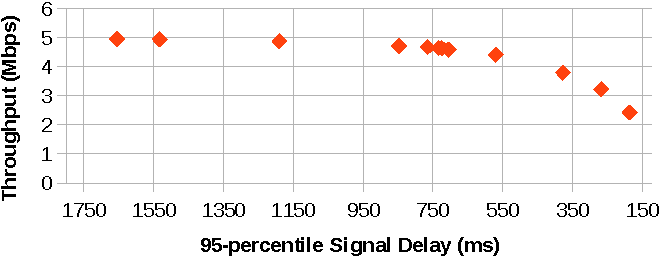
\includegraphics[height=3cm]{./img/exb_fig.pdf}
  \caption{Throughput vs 95-percentile Signal Delay for simple AIMD.}
  \label{fig:exb}
\end{figure}


\vfill
\pagebreak

\section*{Exercise C}
\begin{question}
  Implement a simple delay-triggered scheme, where the window rises or falls
  based on whether the round-trip-time crosses some threshold value. Experiment
  with a few thresholds or tweaks and report on what worked the best.
\end{question}

We implemented a simple scheme that increases or decreases the window size
based on an RTT threshold. On each ACK, we calculate the RTT of the particular
datagram and additively increase the window if the RTT is less than the threshold,
or additively decrease the window size if the measured RTT is
greater than the threshold.
The amount of increase and decrease are defined by the constants
\texttt{alpha} and \texttt{beta}, respectively.

We experiment with several values of our three constants: \texttt{alpha},
\texttt{beta}, and \texttt{rtt\_thresh}, and summarize the results in
Table~\ref{tab:delay}

\begin{table}[h]
  \centering
  \caption{Performance of Delay-based Congestion Control}
  \label{tab:delay}
  \scriptsize
  \begin{tabular}{rrrrrr}
    \toprule
    \textbf{alpha} & \textbf{beta} & \textbf{rtt\_thresh (ms)} & \textbf{\specialcell{Throughput\\(Mbits/s)}} & \textbf{\specialcell{95\% Signal\\Delay (ms)}} & \textbf{Score}\\
    \midrule
    1   & 20     & 100  & 3.30  & 149  & 22.15  \\
    1   & 10     & 100  & 3.76  & 155  & 24.26  \\
    1   & 5      & 100  & 4.32  & 190  & 22.26  \\
    1   & 1      & 100  & 4.81  & 497  & 9.68  \\
    1   & 10     & 150  & 4.43  & 820  & 5.40  \\
    \textbf{1}   & \textbf{10}     & \textbf{90}   & \textbf{3.57}  & \textbf{137}  & \textbf{26.06}  \\
    1   & 10     & 85   & 3.34  & 136  & 24.56  \\
    1   & 10     & 80   & 3.15  & 129  & 24.42  \\
    1   & 10     & 70   & 2.57  & 119  & 21.60  \\
    10  & 10     & 90   & 4.75  & 237  & 20.04  \\
    10  & 1      & 90   & 4.89  & 924  & 5.29   \\
    10  & 1      & 60   & 4.89  & 924  & 5.29   \\
    \bottomrule
  \end{tabular}
\end{table}

We found that using this approach, we achieved the best performance when the
additive decrease occurred at a faster rate than the additive increase in order
to quickly allow the queues to drain when a particular RTT is exceeded to reduce
the queueing delay. We also found that the best RTT threshold was about 90ms,
when combined with our selection of alpha and beta.

\begin{figure}[h]
  \centering
  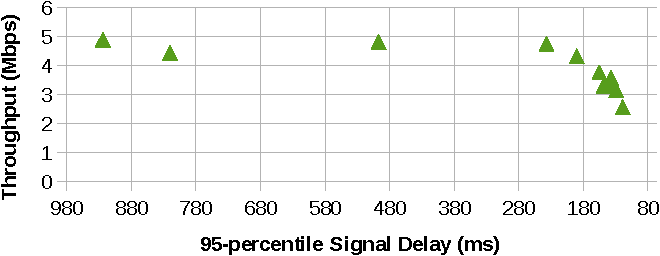
\includegraphics[height=3cm]{./img/exc_fig.pdf}
  \caption{Throughput vs 95-percentile Signal Delay for simple AIMD.}
  \label{fig:exc}
\end{figure}


This approach produced the best score of any of our attempts thus far.
We believe that even a simple-delay based algorithm was able to outperform
AIMD or a fixed window scheme due to it's ability to react to congestion in the
network (by observing RTTs of individual datagrams). In the fixed window scheme,
no adjustments were made for congestion, and in the AIMD scheme of the previous
exercise, the algorithm only reacted to timeouts (since our mahimahi
environment does not drop datagrams). Consequently, AIMD would still cause
bufferbloat during additive increase, and had to wait for timeouts to stop its
growth, rather than the growing queueing delay.

\vfill
\pagebreak

\section*{Exercise D}
\begin{question}
  Try different approaches and work to maximize your score on the final
  evaluation. Be wary about ``overtraining'': after the contest is over, we
  will collect new network traces and then run everybody's entries over the
  newly-collected evaluation trace. In your report, please explain your
  approach, including the important decisions you had to make and how you made
  them. Include illustrative plots.
\end{question}

\subsection*{Attempt 1: EWMA Receiver Rate \& BW}
In our first approach, we referred to the Sprout-
EWMA\footnote{\url{http://alfalfa.mit.edu/}} idea of using an exponentially
weighted moving average to estimate the rate that the receiver was receiving
datagrams. This served as a proxy of the bottleneck bandwidth
capacity and varied over time. We then approximated the RTT to as the minimum
RTT that was seen during the flow.
Then, our algorithm tried to maintain the bandwidth delay product number of
datagrams in flight at any given time as $RTT_{estimate} * BW_{estimate}$ using
the estimates we calculated.

While implementing this approach, we found that there were interesting edge
cases that required us to add minimum and maximum bounds on the window size.
In particular, if no minimum was set, we found that it was possible for our
algorithm to reach a state where the estimated bandwidth was a rate of 1 datagram
per RTT, which caused our algorithm to send a single datagram at a time in an
attempt to avoid bloating the buffers, when really the estimate itself
was incorrect.

This approach used the following parameters:
\texttt{max\_window}, \texttt{min\_window}, and \texttt{weight}.
We initialized our estimated RTT to $80$ ms, and our estimated receiver rate to
1 datagram per 2.4 ms (approximately 5Mbps). The weight is used in updating the
average time between datagrams received by the receiver as
$time = (weight * measured_time) + ((1 - weight) * time)$
where $measured_time$ is the time interval between datagrams received, and the
rate is calculated as $1$ datagram per $time$. This means that a larger weight
gives more influence to the current measurement than past measurements. On
our trace, the estimated RTT converges to the minimum RTT of 42ms.

\begin{table}[!h]
  \centering
  \caption{Performance of EWMA-estimated Rate \& Min RTT}
  \label{tab:attempt_1}
  \scriptsize
  \begin{tabular}{rrrrrr}
    \toprule
    \textbf{max\_window} & \textbf{min\_window} & \textbf{weight} & \textbf{\specialcell{Throughput\\(Mbits/s)}} & \textbf{\specialcell{95\% Signal\\Delay (ms)}} & \textbf{Score}\\
    \midrule
    100   & 0     & 0.25  & 0.01  & 1027  & 0.01  \\
    100   & 2     & 0.25  & 0.43  & 103   & 4.17  \\
    100   & 3     & 0.25  & 2.85  & 199   & 14.32  \\
    100   & 5     & 0.25  & 3.18  & 213   & 14.93  \\
    100   & 3     & 0.50  & 4.28  & 370   & 11.57  \\
    100   & 5     & 0.50  & 4.32  & 362   & 11.93  \\
    100   & 5     & 0.75  & 4.30  & 667   & 11.93  \\
    100   & 5     & 0.10  & 1.16  & 112   & 10.36  \\
    200   & 5     & 0.40  & 3.88  & 1421  & 2.73  \\
    80    & 5     & 0.30  & 3.69  & 218   & 16.93  \\
    \bottomrule
  \end{tabular}
\end{table}

As shown in Table~\ref{tab:attempt_1}, we were unable to break above a power
score of 20. Note that when \texttt{min\_window} was set to 0, we see
dismal scores to do our algorithm getting in the undesirable state of sending
only a single datagram at a time as described above. Furthermore, increasing
this minimum to 2 datagrams resulted in similar behavior, where 1 datagram would be
sent per $RTT/2$, and not provide an accurate feedback signal for our estimates.
Once the minimum window was set to 3 datagrams, we were able to get better
feedback, and break out of the negative feedback states that occurred in the
previous two settings when throughput of the link suddenly dropped
significantly. However, even with this minimum, our algorithm was slow to
recover from these large drops, and would often take 5 or more seconds before
utilizing the available bandwidth.

Ultimately, the primary flaw of this approach is that if the algorithm reached
some steady state at a low throughput, and was unable to quickly break out of
this low-throughput state to utilize the available bandwidth, and when it did
break out of this state, it often overshot the available bandwidth, causing
large queuing delays. We worked to address this in our following attempt.

\subsection*{Rocinante: Delay-Based Additive Increase, Additive Decrease}

We decided build off of the delay-based algorithm from
Exercise C. Specifically we built on the idea of using an additive-increase
and additive decrease. However, unlike the previous attempt, which used a
naive RTT threshold, we now use feedback from the acknowledged datagrams to set
this threshold.

In this algorithm, we use an additive increase (controlled by \texttt{alpha})
and an additive decrease (controlled by \texttt{beta}). At all times, the
algorithm is either increasing cwnd or decreasing it, based on an
exponentially weighted moving average of the RTTs seen, and the current RTT
of a particular datagram. At a high level, when the RTTs being seen are
``stable'', or within a specified range of the average RTT, the congestion
window is additively increased. However, when a RTT is reported that exceeds
this allowance around the average RTT, it signals congestion, and the algorithm
decreases the congestion window to avoid bloating the bottleneck queues.
When the network is congested, the exponentially weighted moving average is
also reset to the estimated round trip propagation time, which serves as a
baseline of the expected RTT in an non-congested network.

Several observations motivated the design of this algorithm. First, we learned
from Exercise A, B, and C, that in general, an algorithm that reacts to delay
rather than datagram loss or timeout is able to respond to congestion much more
quickly, and is able to keep the queues relatively small.
Second, from our first attempt, we realized that our algorithm must be able
to avoid getting stuck in an undesirable stable state. In our case, we saw
that having two simple states (increasing or decreasing) was an intuitive way
ensure that the algorithm was responsive. This was just a choice we made for
simplicity, other algorithms like BBR use more complex states (e.g. ProbeBW) to
ensure that the available throughput is utilized.

With this general design of our algorithm in place, we moved on to testing the
performance of our various parameters: (1) \texttt{alpha}, which defines the
amount of additive increase to apply to cwnd; (2) \texttt{beta}, which defines
the amount of additive decrease for cwnd; (3) \texttt{rtt\_allowance}, which
defines how much a RTT measurement is allowed to exceed the average RTT while
still being considered ``stable''; (4) \texttt{ewma\_weight}, which defined
the weight applied to the current measurement of RTT in the EWMA of RTT; and
\texttt{timeout}, which defined the RTO in milliseconds before another datagram
is sent. The some of the results of our exploration are shown in
Table~\ref{tab:rocinante}.

\begin{table}[h]
  \centering
  \caption{Performance of Rocinante (Delay-based AIAD)}
  \label{tab:rocinante}
  \scriptsize
  \begin{tabular}{rrrrrrrr}
    \toprule
    \textbf{alpha} & \textbf{beta} & \textbf{rtt\_allowance} & \textbf{ewma\_weight} & \textbf{timeout} & \textbf{\specialcell{Throughput\\(Mbits/s)}} & \textbf{\specialcell{95\% Signal\\Delay (ms)}} & \textbf{Score} \\
    \midrule
    1  & 2  & 1.4 & 0.15  & 1000 & 4.94 & 2064 & 2.39 \\
    1  & 4  & 1.4 & 0.15  & 1000 & 4.85 & 1902 & 2.54 \\
    1  & 5  & 1.4 & 0.15  & 1000 & 4.85 & 1896 & 2.56 \\
    1  & 10 & 1.4 & 0.15  & 1000 & 4.67 & 1788 & 2.61 \\
    2  & 5  & 1.4 & 0.15  & 1000 & 4.98 & 2807 & 1.77 \\
    2  & 5  & 1.4 & 0.01  & 1000 & 3.25 & 120  & 27.08 \\
    2  & 5  & 1.4 & 0.00  & 1000 & 2.92 & 114  & 25.61 \\
    5  & 2  & 1.4 & 0.01  & 1000 & 4.71 & 1853 & 2.54 \\
    2  & 5  & 1.1 & 0.01  & 1000 & 0.42 & 111  & 3.78 \\
    2  & 5  & 1.5 & 0.01  & 1000 & 4.00 & 643  & 6.22 \\
    2  & 5  & 1.4 & 0.01  & 100  & 3.29 & 105  & 31.33 \\
    2  & 5  & 1.4 & 0.01  & 50   & 3.24 & 83   & 39.04 \\
    2  & 5  & 1.4 & 0.01  & 25   & 3.47 & 86   & 40.35 \\
    2  & 5  & 1.4 & 0.01  & 15   & 3.55 & 98   & 36.22 \\
    \bottomrule
  \end{tabular}
\end{table}

From our experiments, and by observing the behavior of the throughput and
queueing delay graphs paired with debug outputs, we saw that out initial
choice of EWMA weight ($0.15$) allowed the average to drift too quickly, and
thus allowed the algorithm to bloat the buffers. Instead, lowering this weight
such that the average stayed relatiely close to our estimate of the propagation
delay significantly reduced the 95-percentile signal delay. However, we also
found that eliminating the weight entirely could negatively affect our score.
An alternative approach may have been to eliminate the EWMA average and use
some statistical variance to determine what RTT's to consider ``stable'', but
we did not explore this alternative.

Next, we found that it was important in our AIAD algorithm to ensure that
additive decrease occurred at a rate that was faster than additive increase.
Intuitively, this allows the algorithm to more quickly close the window when
congestion is detected. If we used an even more aggressive decrease (e.g.
exponential), we found that throughput was wasted as just a few decreases could
almost completely close the window.

When we experimented with the RTT allowance, which defines how much a measured
RTT can exceed the average while still being considered ``stable'', we initially
selected a vale of $1.4$ due to our observations from an experiment with a
fixed window size of 1 datagram. In particular, we saw that the minimum RTT was
42 ms, and that individual packet RTTs could vary significantly from about 40ms
up to about 60ms. Further experiments with a small allowance shows that small
allowance is too limiting, and hurts throughput performance. Consequently, we
selected an allowance of about $1.4$ (i.e. a measured RTT value that is $1.4\times$
larger than the average can be considered stable). This seemed to work well due
the nature of the cellular network trace, which resulted in large ($>1.4\times$)
spikes in RTT when the throughput of the link dropped. Similar to the RTT
average, the purpose of this is just to define what a ``stable'' RTT looks like,
and an alternative approach could be using statistics on the RTTs seen, rather
than a fixed allowance as we have implemented here.

We found that tuning the first four parameters resulted in a score of slightly
less than 30, but we were unable to exceed this. Unexpectedly, lowering the
timeout value significantly improved our score. We suspect that this is due to
our initial misunderstanding of ``signal delay''. We had previously assumed
that we were trying to minimize the delay of individual datagrams. However,
``signal delay'' is also negatively affected by dead time, when no datagrams
are being sent. By lowering timeout, we ensure that there is a minimum trickle
of datagrams being sent, as a rate that is low enough to not negatively bloat
buffers, but frequently enough to ensure that our signal delay is not affected
by seconds of dead time.

Overall, our algorithm was most sensitive to changes to the RTT allowance, EWMA
weighting, and timeout. The choice of alpha and beta had less affect as long as
both values were relatively small, and beta was larger than alpha.

\begin{figure}[h]
  \centering
  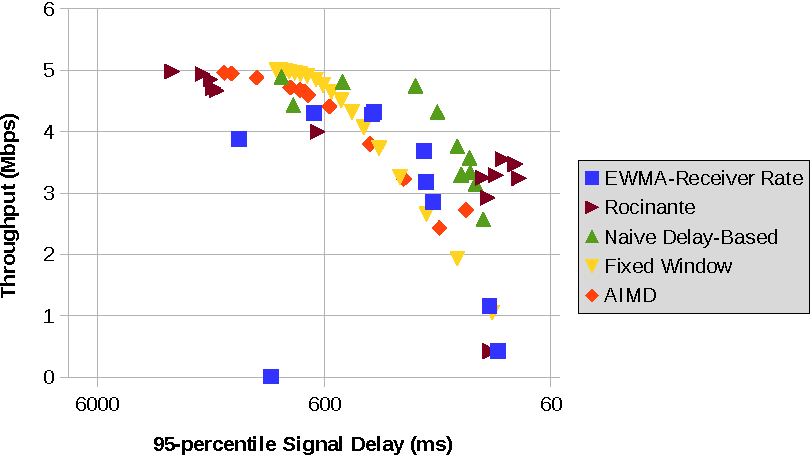
\includegraphics[height=7cm]{./img/total.pdf}
  \caption{Throughput vs 95-percentile Signal Delay for all Exercises.
  We found that delay-based schemes produced the highest score and improved
  on our algorithm from Exercise C for Exercise D.}
  \label{fig:all_attempts}
\end{figure}

As a comparison, we show attempts from each of the exercises all together in
Figure~\ref{fig:all_attempts}. Much like the congestion control competition
itself, we were also able to explore the various realizable algorithms within
the Pareto frontier. We noticed that using this enhanced delay-based AIAD
approach allowed us to significantly reduce the 95-percentile signal delay
while maintaining reasonable throughput than our other attempts, which lead
to the best power scores.

\pagebreak

\begin{figure}[t]
  \centering
  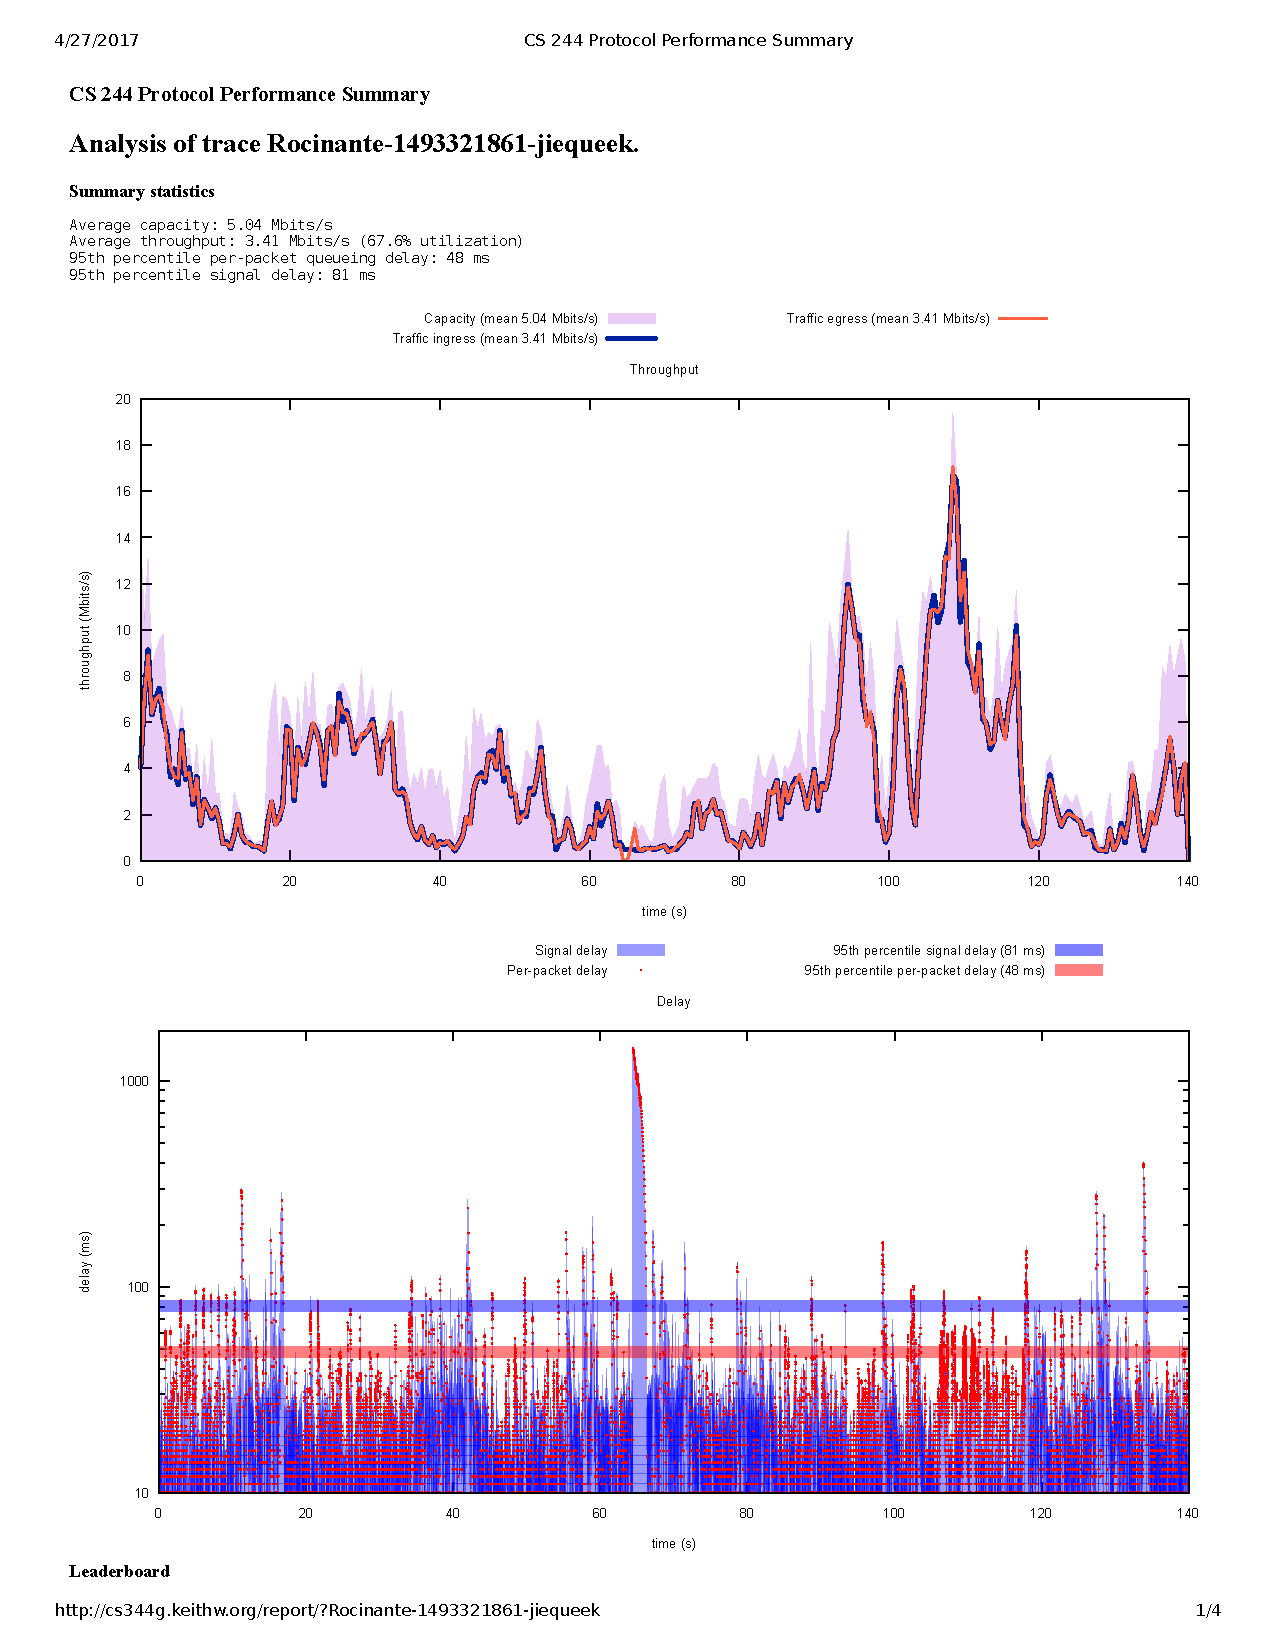
\includegraphics[height=7cm, clip, trim={1cm 12cm 1cm 6cm}]{./img/final_trace.pdf}
  \caption{Rocinante on the Verizon trace (alpha = 2, beta = 5,
    rtt\_allowance = 1.4, ewma\_weight = 0.01, and timeout = 25)
  }
  \label{fig:final_trace}
\end{figure}

In Figure~\ref{fig:final_trace}, we see that our algorithm is conservative, in
that it often does not fully utilize the available bandwidth. Furthermore,
because we are simply doing additive increase, we see that our algorithm can
also be a little but slow to grow. For example, at about 70 seconds into the
trace, available bandwidth increases, but our algorithm additively increases
its congestion window and misses out on some of the available throughput.
One approach that may have addressed this would be to implement a short probing
state like that in BBR, where BBR can converge exponentially fast to a new
bottleneck bandwidth.

\begin{figure}[h]
  \centering
  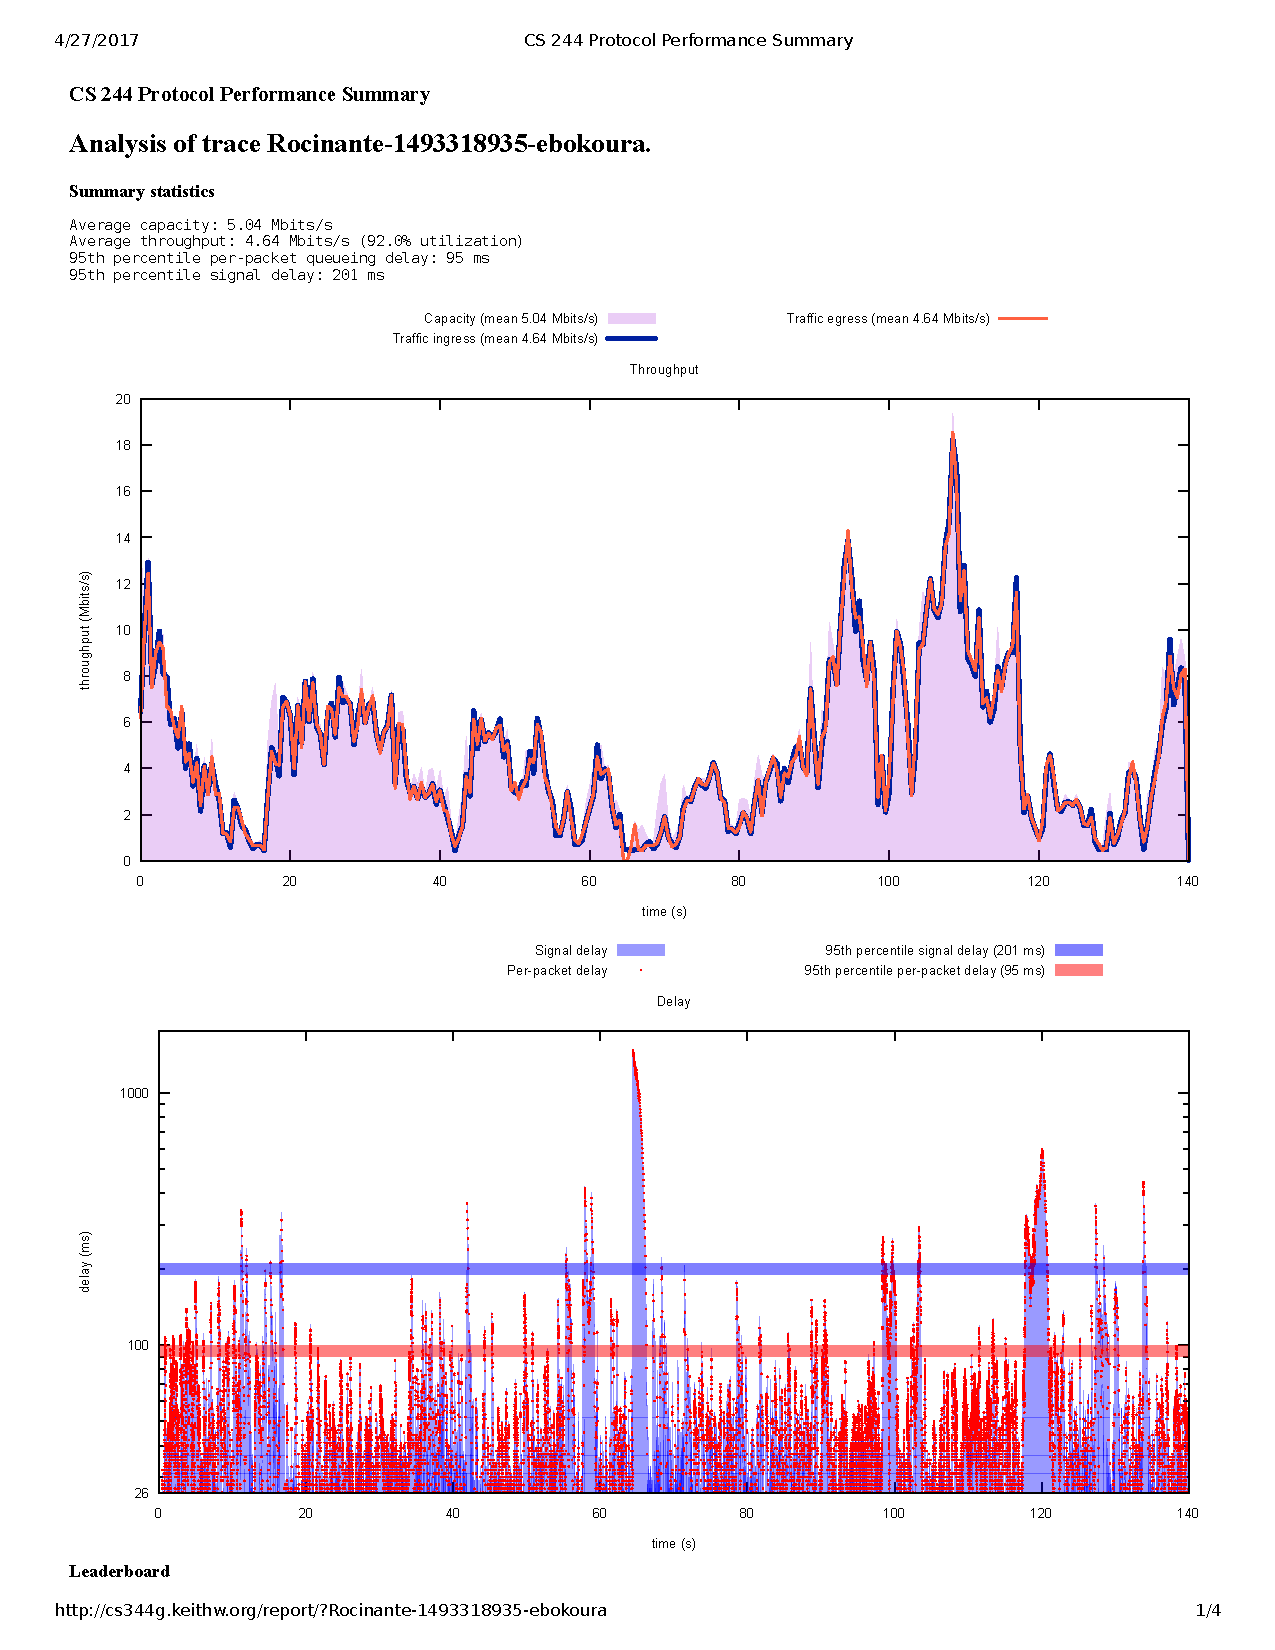
\includegraphics[height=7cm, clip, trim={1cm 12cm 1cm 6cm}]{./img/a5b2.pdf}
  \caption{Rocinante on the Verizon trace (alpha = 5, beta = 2,
    rtt\_allowance = 1.4, ewma\_weight = 0.01, and timeout = 25)
  }
  \label{fig:a5b2}
\end{figure}

In contrast, Figure~\ref{fig:a5b2} shows the behavior of Rocinante when
alpha = 5 and beta = 2. Notice that by just tweaking the algorithm such that
additive increase occurs faster than additive decrease, the algorithm is much
more aggressive, and quicker to fill the available. However, as a result, this
results in much higher 95-percentile signal delay and a score of about 23.
We used these throughput graphs to visually get a sense of the behavior of
our algorithm at various parameter settings, in order to know how to adjust
the parameters to improve our overall score.

\vfill
\pagebreak

\section*{Exercise E}
\begin{question}
  Pick a cool name for your scheme!
\end{question}

We call our approach \texttt{Rocinante}, named after the light, agile attack
ship in The Expanse. Our code is available on GitHub here:

\begin{center}
  \fbox{\parbox{10cm}{\centering
  \url{https://github.com/jervisfm/cs244-project2}
  }}
\end{center}


\subsection*{Summary Statistics}
As requested in the submission guidelines, our final submission's summary
statistics are shown below.
\begin{center}
  \fbox{\parbox{10cm}{
  Average capacity: 5.04 Mbits/s \\
  Average throughput: 3.31 Mbits/s (65.6\% utilization) \\
  95th percentile per-packet queueing delay: 39 ms \\
  95th percentile signal delay: 79 ms \\
  \textbf{Power Score: 41.90}
  }}
\end{center}




% =============================================================================
\end{document}
